% !TeX root = ../../main.tex
\newpage
\section{Generator sztucznych danych}
\label{sec:generator}

Problem skompletowania dostatecznie licznego zbioru treningowego został rozwiązany poprzez stworzenie generatora sztucznych obrazów.
Generator, zaimplementowany jako scena 3D w JavaScript pozwala na generowanie obrazów z~następującymi cechami:

\begin{itemize}
	\item zmienne kolory obiektów: podłogi, kortu, słupków;
	\item dynamiczne światło;
	\item zmienna pozycja zawodników;
	\item zmienne odległości między kortami.
\end{itemize}

Dzięki powyższym cechom możliwe jest przygotowanie sztucznych obrazów zbliżonych do obrazów z kamer przemysłowych stosowanych na meczach odbywających się w różnych lokalizacjach.

W celu, aby obraz stanowił rekord treningowy, wymagana jest tak zwana anotacja, czyli oznaczenie obszaru kortu. Do anotacji wykorzystano program \textit{VGG Image Annotator} \cite{dutta2016via} \cite{dutta2019vgg}.
\\
Zbiór danych treningowych złożony z wygenerowanych sztucznych danych zawiera 72 obrazy o rozdzielczości 800x600 pikseli.

\begin{figure}[!htb]
  \minipage{0.45\textwidth}
    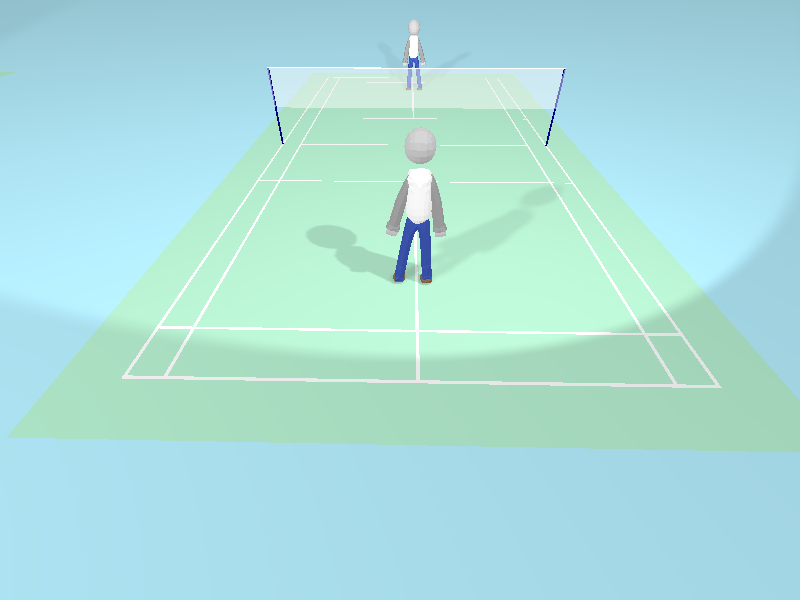
\includegraphics[width=\linewidth]{./fake.jpg}
    \caption{Przykład wygenerowanego sztucznego obrazu}
  \endminipage\hfill
  \minipage{0.45\textwidth}
    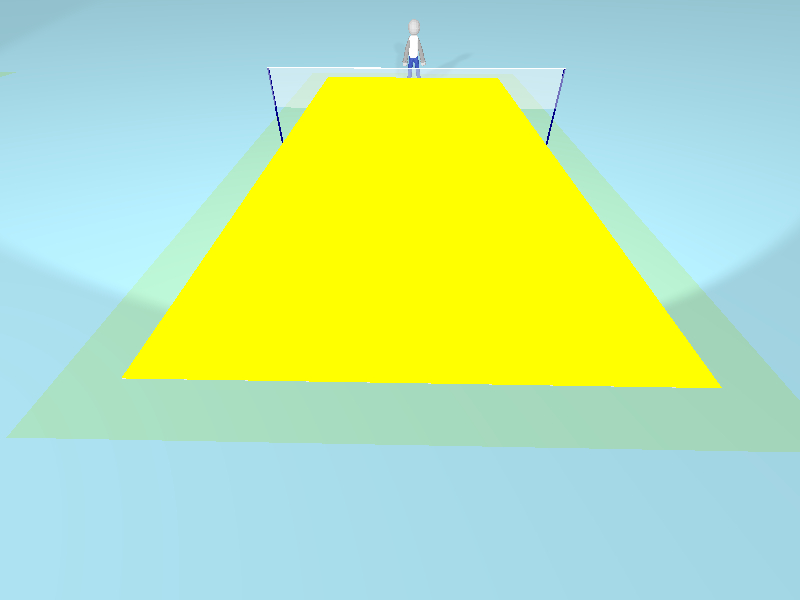
\includegraphics[width=\linewidth]{./fake_annotated.jpg}
    \caption{Sztuczny obraz z zaznaczoną na żółto anotacją powierzchni kortu}
  \endminipage\hfill
\end{figure}
